\section{Machine Learning Fundamentals}\label{sec:ml-fundamentals}
This chapter provides the machine learning background for the remainder of the thesis. It begins with the terminology of neural networks and their training. The chapter then focuses on recurrent architectures and the long short-term memory (LSTM) cell. The generative adversarial network (GAN) is introduced next, followed by its conditional, forecasting and financial variants.

\subsection{Neural Networks}\label{sec:nn}
Feedforward neural networks are a class of machine learning models that define a mapping $y=f(x;\theta)$, where $x$ is the input, $y$ is the output, and $\theta$ are the learnable parameters. The model is a composition of functions 
\begin{equation}
f(x) = f^{(L)}\!\left(\cdots f^{(2)}\!\left(f^{(1)}(x)\right)\cdots\right),
\label{eq:nn-composition}
\end{equation}
where $f^{(L)}$ is the output layer, and $L$ is the depth of the network. $f^{(1)}$, $f^{(2)}$, $\dots$, $f^{(L-1)}$ are referred to as the hidden layers. The dimensionality of the hidden layers is called their width. Computing $f(x)$ by evaluating the functions in order is called forward propagation.

Several types of layers exist, including fully connected, convolutional, and recurrent layers. Only fully connected layers, also called dense layers, and recurrent layers are used in this thesis. Recurrent layers are described in Sec.~\ref{sec:rnn}. In a dense layer, the input is multiplied by a weight matrix $W$ and a bias vector $b$ is added. The operation is linear, so a composition of linear functions would again be linear. A nonlinear activation function $g$ is applied to the output
\begin{equation}
f^{(i)}(x) = g\!\left(W^{(i)} x + b^{(i)}\right).
\end{equation}
The weights and biases of all layers form the learnable parameters $\theta$. Rectified linear unit (ReLU) and sigmoid are two commonly used activation functions. ReLU is defined as $g(x) = \max(0,x)$, and sigmoid is defined as $g(x) = 1/(1+\exp(-x))$. Sigmoid is often used in the output layer for binary classification to map the output to $(0,1)$. ReLU is often used in the hidden layers \parencite[ch.~6]{goodfellowDeepLearning2016}.

\subsubsection{Training}\label{sec:nn-training}

Training is a process of finding parameters $\theta$ that fit the model to a set of examples, called training data. Learning problems are generally categorized as supervised and unsupervised.
In supervised learning, the model learns a mapping from input to output using labeled data. Labeled data consists of input-output pairs, where the output is the target value. In unsupervised learning, the data is unlabeled and the model learns the probability distribution that produced it.

The parameters $\theta$ must be chosen so that the model fits the training data. The cost function measures how badly the model performs on the training data. In supervised learning, it measures the difference between the model output and the target value. In unsupervised learning, it measures how poorly the model's distribution matches the data. Training minimizes the cost function with respect to $\theta$. 

Classification is a supervised learning problem where the model predicts which category each input belongs to. These categories are called classes. In binary classification there are two classes. Cross-entropy is a commonly used cost function for binary classification. This cost function is defined as 
\begin{equation}
   J(\theta) = -\frac{1}{n}\,\sum_{i=1}^{n}[y_i\log(\hat{y}_i) + (1-y_i)\log(1-\hat{y}_i)],
\end{equation}
where $n$ is the number of training examples, $y_i \in \{0,1\}$ is the true class and $\hat{y}_i$ is the predicted probability. $J$ is small when the predicted probability is close to the true class. $J$ grows without bound as the predicted probability approaches the opposite class.

The gradient $\nabla_{\theta}J$ is the vector of partial derivatives of $J$ with respect to $\theta$. $\nabla_{\theta}J$ points in the direction of the greatest increase of $J$. Moving in the direction of the negative $\nabla_{\theta}J$ decreases $J$. This procedure is called gradient descent. Each step of gradient descent updates the parameters $\theta$ according to
\begin{equation}
\theta' = \theta - \eta \nabla_{\theta}J,
\end{equation}
where $\eta$ is the step size, called the learning rate. The step is repeated until the cost stops decreasing. Backward propagation computes the gradient of $J$ with respect to $\theta$ by applying the chain rule to the composition in Eq.~\eqref{eq:nn-composition}.
The norm of a vector is a measure of its length. The gradient norm measures the magnitude of $\nabla_{\theta}J$ and is defined as
\begin{equation}
\|\nabla_{\theta}J\| = \sqrt{\sum_{i=1}^{d}\left(\frac{\partial J}{\partial \theta_i}\right)^2},
\end{equation}
where $d$ is the number of parameters in $\theta$. Computing the gradient over the entire training data is computationally expensive. Instead, the training data is divided into subsets called minibatches. The gradient is computed, and the parameters are updated for each minibatch. The minibatches are drawn randomly, so each gradient is a noisy estimate of the gradient over the full training data. This is called stochastic gradient descent (SGD). One pass over the entire training data is called an epoch. The training data is shuffled at the start of each epoch, so that the minibatches differ between epochs.

The cost function of a neural network is generally non-convex. A function is convex if it has a single global minimum, while non-convex functions have multiple local minima. Gradient descent may converge to a local minimum, which may not be the global minimum. Neural networks are trained with optimizers, variants of gradient descent that adapt the step size during the training process. RMSProp is an example of such an optimizer. It divides the learning rate by a running average of the squared partial derivatives for each parameter. As a result, each parameter has its own effective learning rate. 

The initial values of the parameters $\theta$ affect the convergence of the training process. If the initial values are too small, the gradients become very small, and the training process is slow. If the initial values are too large, the gradients grow and the training process diverges. Two commonly used initialization methods are Xavier \parencite{xavier-init} and He initialization \parencite{heDelvingDeepRectifiers2015}. Both methods draw the initial values from a normal distribution with mean zero. The standard deviation differs between the two methods
\begin{equation}
s_{\text{Xavier}} = \sqrt{\frac{2}{n_{\text{in}} + n_{\text{out}}}}, \qquad
s_{\text{He}} = \sqrt{\frac{2}{n_{\text{in}}}},
\end{equation}
where $n_{\text{in}}$ and $n_{\text{out}}$ are the input and output dimensions of the layer.

Apart from learnable parameters $\theta$, neural networks have hyperparameters that are set before training. Hyperparameters include the learning rate, the number of epochs, the minibatch size and the width of the layers. They are not learned during training, but they affect the training process and the final model. Hyperparameters are chosen by experiment. 

The capacity of a neural network is its ability to represent a wide range of functions. Adding more layers to the model or increasing the width of the layers increases the capacity. A model with insufficient capacity underfits. Underfitting occurs when the model's output does not fit the training data well. A model with excessive capacity is prone to overfitting. Overfitting occurs when the model fits the training data closely but performs poorly on unseen data.

\subsubsection{Recurrent Neural Networks and LSTM}\label{sec:rnn}

Time series data is an ordered sequence: the position of each value in the sequence carries information. A dense layer has separate parameters for each input position. What a dense layer learns from one position does not transfer to other positions. A recurrent layer processes a sequence of values, using the same parameters $\theta$ for each position. A neural network consisting of recurrent layers is called a recurrent neural network. Recurrent layers are updated sequentially, one step at a time. At each step, a recurrent layer takes the current input and a hidden state carried from the previous step to produce the output and the next hidden state
\begin{equation}
h^{(t)} = f\!\left(h^{(t-1)}, x^{(t)}; \theta\right),
\end{equation}
where $h^{(t)}$ is the hidden state at step $t$ and $x^{(t)}$ is the input at step $t$. The final hidden state is a fixed-length vector representation of the entire sequence, where $T$ is the length of the sequence. The dimension of the hidden state is called the hidden size of the recurrent layer and determines the capacity of the layer. The hidden size is a hyperparameter that is set before training.

In a recurrent layer, the gradient $\nabla_{\theta}J$ is propagated backward through every step of the sequence. The same parameters $\theta$ are applied at each step, so $\nabla_{\theta}J$ is multiplied by the same factor at each step. As a result, $\nabla_{\theta}J$ can grow without bound or vanish to zero over long sequences. This is commonly called the  vanishing and exploding gradient problem.

The long short-term memory (LSTM) cell \parencite{hochreiterLongShortTermMemory1997} addresses the vanishing and exploding gradient problem. It introduces a memory cell $c^{(t)}$, carried alongside the hidden state. Three gates with entries in $(0, 1)$ control the memory cell. They determine how much of the memory cell is retained, how much of the current input is stored in the memory cell, and how much of the memory cell is passed to the output. The memory cell is updated by addition, so the gradient can flow through many steps without vanishing. The gated recurrent unit (GRU) \parencite{choLearningPhraseRepresentations2014} is a related gated architecture.
\subsection{Generative Adversarial Networks}
Generative modeling is an unsupervised learning approach (Sec.~\ref{sec:nn-training}). A generative model takes a set of training examples and learns the probability distribution that produced them. GANs are generative models first introduced by \textcite{goodfellowGenerativeAdversarialNetworks2014}.
GANs have been particularly successful in image and video generation. They have also been used to create synthetic data, for training other machine learning models and to fill in gaps in missing data \parencite{goodfellowGenerativeAdversarialNetworks2020}.

\subsubsection{Basic Generative Adversarial Networks}\label{sec:basic-gan}

GANs are based on game theory, which studies situations where several decision-makers are present. Each participant chooses an action, and the outcome depends on the choices of all participants. A GAN has two decision-makers, the generator $G$ and the discriminator $D$, typically implemented as neural networks. $G$ takes a vector of random noise as input and generates a sample as output. $D$ takes a real or generated data sample as input and outputs a probability that the input sample is real. The goal of $G$ is to fool $D$ by generating realistic samples. The goal of $D$ is to distinguish real samples from generated ones.

Assume that the data $x$ follows an unknown distribution $p_{data}$, from which new samples need to be generated. The generator is a neural network $G(z; \theta_g)$, where $\theta_g$ denotes the learnable parameters. The input $z$ is a noise vector drawn from a prior distribution $p_z$. Gaussian distribution is normally used to define $p_z$; the GAN framework does not add limitations. The probability distribution of the generated samples is denoted $p_g$. The discriminator is a neural network $D(x; \theta_d)$, with learnable parameters $\theta_d$. It outputs the estimated probability that the input was drawn from  $p_{data}$ rather than $p_{g}$. $G$ and $D$ have cost functions, respectively $J^{(G)}(\theta_d, \theta_g)$ and $J^{(D)}(\theta_d, \theta_g)$. Both $G$ and $D$ need to minimize their cost functions, while they can only control their learnable parameters, respectively $\theta_g$ and $\theta_d$. Hence, the solution is a Nash equilibrium, rather than a minimum of a single cost function.

The GAN framework is flexible in the sense of the cost functions applied to $G$ and $D$. The simplest version of the game is a zero-sum game. In this, the sum of all of the cost functions is always zero.
\begin{equation}
J^{(G)}(\theta_d, \theta_g) = -J^{(D)}(\theta_d, \theta_g).
\end{equation}

The cost function of $D$ is defined as a standard cross-entropy (Sec.~\ref{sec:nn-training})
\begin{equation}
J^{(D)}\bigl(\theta_d, \theta_g\bigr)
= -\frac{1}{2}\,\mathbb{E}_{x \sim p_{\text{data}}} \log D(x)
  - \frac{1}{2}\,\mathbb{E}_{z} \log\bigl(1 - D\bigl(G(z)\bigr)\bigr).
\end{equation}

Learning the zero-sum game minimizes the Jensen-Shannon divergence between $p_{\mathrm{data}}$ and $p_g$. Convergence holds only if both players are updated in function space. In function space $D$ and $G$ are updated freely among all possible functions. In practice, $D$ and $G$ are neural networks and updated in parameter space. In parameter space the reachable functions are limited to those the network architecture can represent. $D$ minimizes a cross-entropy while $G$ maximizes the same quantity. Generated samples are rejected with high confidence at the start of training, and the gradient of $G$ vanishes at the point at which it performs worst \parencite{goodfellowNIPS2016Tutorial2017}.

Therefore, the cost function of $G$ is constructed by flipping the target of the cross-entropy.

\begin{equation}
J^{(G)}(\theta_d, \theta_g)
= -\frac{1}{2}\,\mathbb{E}_{p_{z}}
  \bigl[\log[D(G(z;\theta_g);\theta_d)]\bigr].
  \label{eq:generator-cross}
\end{equation}

The cost function of $D$ and $G$ do not sum to zero anymore, hence the game is no longer zero-sum. Alternative cost functions have been introduced over time.

Fig.~\ref{fig:standard-gan} is the visualization of a standard GAN workflow adapted from \textcite{vuleticFinGANForecastingClassifying2024}.

\begin{figure}[htbp]
    \centering
    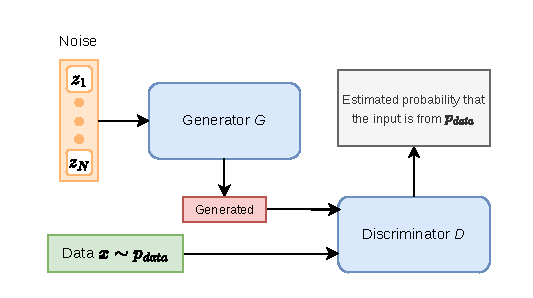
\includegraphics[width=0.7\textwidth]{figures/basic_gan.pdf}
    \caption{Structure of a standard GAN}
    \label{fig:standard-gan}
\end{figure}

GANs are trained by updating the two networks in turn. At each step, a minibatch of samples and noise vectors are drawn from $p_{\mathrm{data}}$ and $p_z$ respectively. $D$ is updated with respect to $\theta_d$ while $\theta_g$ is fixed. $G$ is updated with respect to $\theta_g$ while $\theta_d$ is fixed. $D$ is commonly trained $k$ times for every update of $G$, although \textcite{goodfellowNIPS2016Tutorial2017} argues that $k=1$ is sufficient. $k$ is defined as an independent training parameter. The update cycle is shown in Fig.~\ref{fig:gan-update-cycle}.

\begin{figure}[htbp]
    \centering
    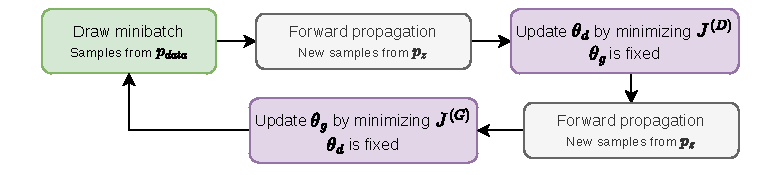
\includegraphics[width=0.9\textwidth]{figures/gan_update_cycle.pdf}
    \caption{Alternating update cycle of a GAN. One $D$ update is performed per $G$ update ($k=1$).}
    \label{fig:gan-update-cycle}
\end{figure}

As stated previously, convergence is not guaranteed in practice. This means that the training of a GAN can settle in a state where $p_g \neq p_{\mathrm{data}}$. The most common such state is mode collapse. It occurs when $G$ repeatedly maps noise vector to very similar outputs. As a result, $p_g$ covers only a small part of $p_{\mathrm{data}}$ but $D$ assigns a high probability that the generated samples are real. Mode collapse is still an unresolved challenge in GAN training. In recent years, several strategies have been proposed to mitigate its effect, such as stronger generators and discriminators, longer training and regularization. However, each of these approaches comes with drawbacks \parencite{barshaIndepthReviewAnalysis2025}.

\subsubsection{cGANs}
Standard GANs can be extended to conditional models \parencite{goodfellowGenerativeAdversarialNetworks2014}. This extension was further developed by \textcite{mirzaConditionalGenerativeAdversarial2014}. In Conditional Generative Adversarial Networks (cGANs), the data follow a conditional distribution $p_{\mathrm{data}}(x \mid \mathrm{c})$, where $c$ is auxiliary deterministic information. The condition is applied to $D$ and $G$ as an additional input.
The cost functions for $G$ and $D$ are the same as for a standard GAN with the condition $c$.

\begin{equation}
J^{(D)}\bigl(\theta_d, \theta_g\bigr)
= -\frac{1}{2}\,\mathbb{E}_{x \sim p_{\text{data}}} \log D(x\mid c)
  - \frac{1}{2}\,\mathbb{E}_{z} \log\bigl(1 - D\bigl(G(z\mid c)\bigr)\mid c\bigr).
\end{equation}

Fig.~\ref{fig:cgan} is the visualization of a cGAN workflow adapted from \textcite{vuleticFinGANForecastingClassifying2024}.

\begin{figure}[htbp]
    \centering
    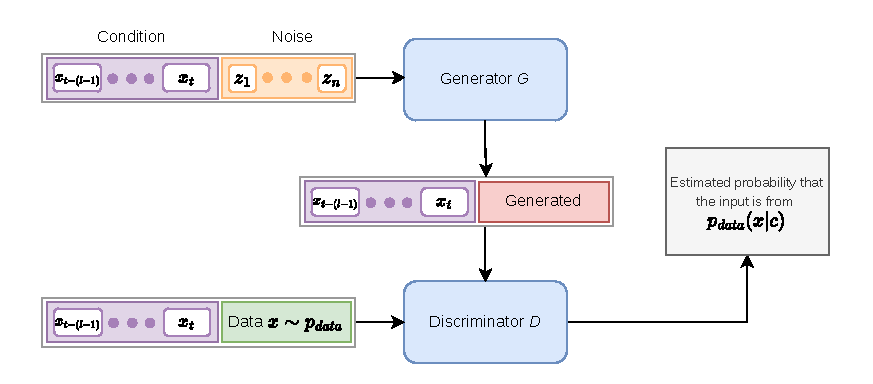
\includegraphics[width=\textwidth]{figures/cgan.pdf}
    \caption{Structure of a cGAN}
    \label{fig:cgan}
\end{figure}


\subsubsection{ForGAN}\label{sec:forgan}
The conditional input proposed in cGANs by \textcite{mirzaConditionalGenerativeAdversarial2014} prepared the ground for domain-specific GAN architectures. ForGAN was introduced specifically for time series forecasting \parencite{koochaliProbabilisticForecastingSensory2019}.

ForGAN is trained to approximate the conditional distribution of the next value in a time series. The condition is the sequence of the previous $l$ observations, ending at time~$t$

\begin{equation}
c = (x_{t-(l-1)}, \ldots, x_t).
\end{equation}

A sliding window of $l+1$ observations is moved along the series. At each position, the first $l$ observations form $c$ and the last is $x_{t+1}$.
$G$ takes a noise vector $z$ and $c$ and outputs a value for the target $x_{t+1}$. $D$ takes a value of $x_{t+1}$ and $c$ and outputs the probability that $x_{t+1}$ is from $p(x_{t+1}\mid c)$. 

A full probabilistic distribution of $x_{t+1}$ can be obtained through repeated sampling of $G$ with different noise vectors and the same $c$.

ForGAN adds a recurrent layer (Sec.~\ref{sec:rnn}) to $G$ and $D$. The layer processes $c$ as an ordered sequence and constructs a vector representation. The recurrent layer can be an LSTM or a GRU (Sec.~\ref{sec:rnn}). The high-level architecture of the ForGAN model is shown in Fig.~\ref{fig:forgan_architecture}.

\begin{figure}[htbp]
  \centering
  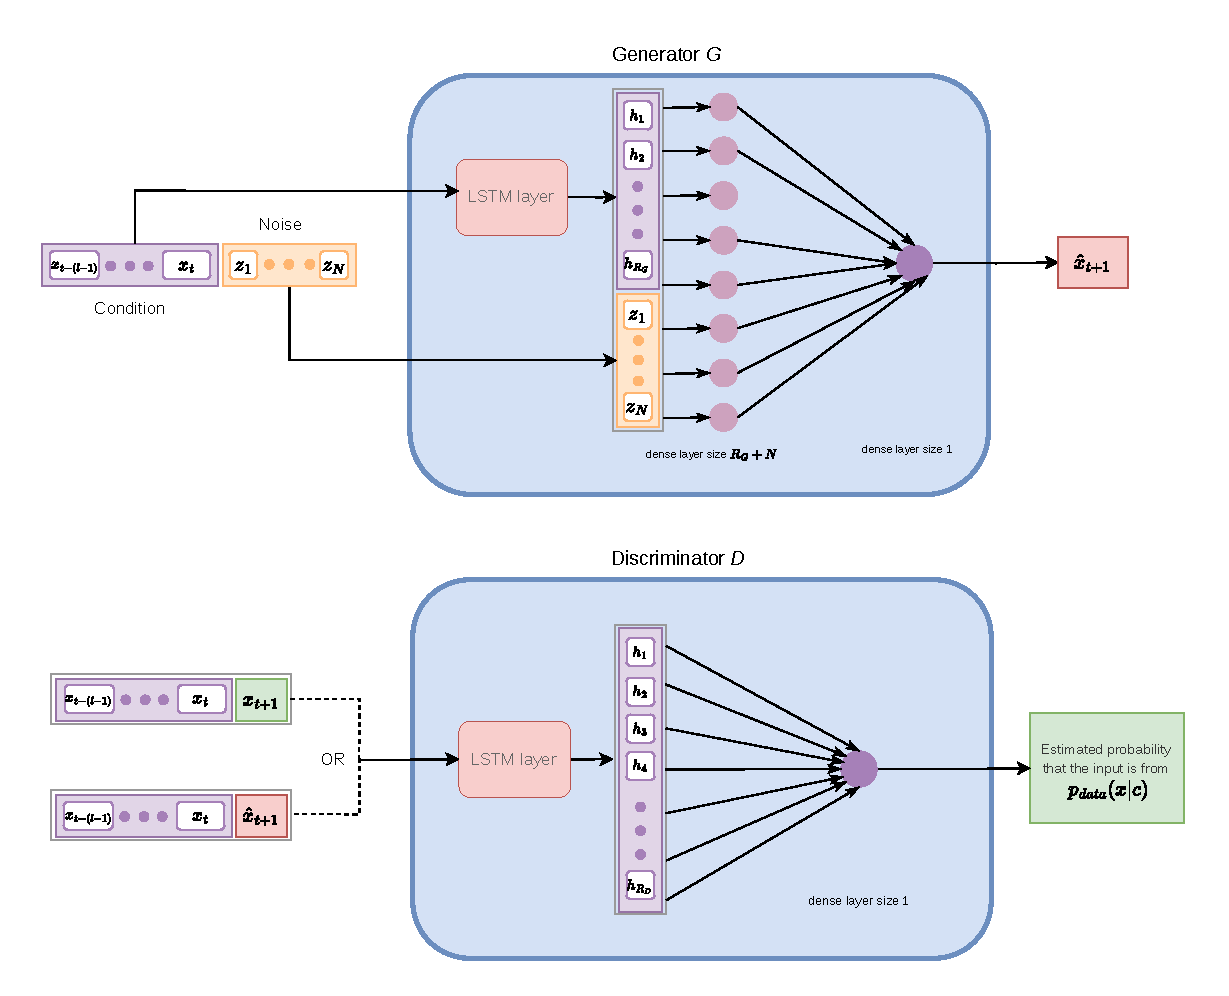
\includegraphics[width=\textwidth]{figures/forgan_architecture.pdf}
  \caption{Structure of a ForGAN}
  \label{fig:forgan_architecture}
\end{figure}

\clearpage
\subsubsection{Fin-GAN}\label{sec:fin-gan}
Fin-GAN was introduced as an extension of ForGAN \parencite{vuleticFinGANForecastingClassifying2024}. It focuses on the probabilistic forecasting of financial time series, specifically equity returns. The ForGAN architecture and the cost function of $D$ are unchanged. LSTM is chosen as the recurrent layer. 

The motivation behind Fin-GAN is to correctly forecast the sign of the return, since the sign determines whether the trade is profitable. For this purpose, economics-driven terms are introduced into the cost function of $G$. In contrast to the unsupervised setting of standard GANs, \textcite{vuleticFinGANForecastingClassifying2024} classify Fin-GAN as supervised learning.

The terms are defined over a minibatch of $n_{\text{batch}}$ pairs. For each condition in the batch, G produces a forecast $\hat{x}_i$ of the realized value $x_i$. Let $\hat{x}=(\hat{x}_1, \ldots, \hat{x}_{n_{\text{batch}}})$ and $x=(x_1, \ldots, x_{n_{\text{batch}}})$. 

\textbf{Cost function.} $J^{(G)}$ can be the zero-sum, cross-entropy or Wasserstein cost function. The latter replaces the Jensen–Shannon divergence between $p_{\mathrm{data}}$ and $p_g$ with the Wasserstein-1 distance \parencite{arjovskyWassersteinGAN2017}. \textcite{vuleticFinGANForecastingClassifying2024} report that the Wasserstein cost function was numerically unstable during training. Hence, $J^{(G)}$ is the cross-entropy cost function given in Eq.~\eqref{eq:generator-cross}. In addition, Fin-GAN introduces four economics-driven terms to the cost function. These are defined below. 

\begin{equation}
L^{G}(x, \hat{x}) = J^{(G)}(x, \hat{x})
- \alpha\,\mathrm{PnL}^{*}_{a}(x, \hat{x})
+ \beta\,\mathrm{MSE}(x, \hat{x})
- \gamma\,\mathrm{SR}^{*}(x, \hat{x})
+ \delta\,\mathrm{STD}(x, \hat{x}).
\label{eq:fingan-loss}
\end{equation}

A positive forecast corresponds to buying an asset, and a negative forecast to selling it short. The profit and loss $\mathrm{PnL}$ of the trade is the sign of the forecast multiplied by the realized return $\mathrm{PnL}(x_i, \hat{x}_i)=\mathrm{sgn}(\hat{x}_i)\cdot x_i$. Since only the sign enters the formula, the outcome does not depend on the magnitude of the forecast. $\mathrm{sgn}(\hat{x}_i)$ is not differentiable, so the standard term $\mathrm{PnL}$ would not provide a gradient for training. A smooth approximation is introduced
\begin{equation}
\mathrm{PnL}^{*}_{a}(x_i, \hat{x}_i) = \tanh(k_{\tanh}\,\hat{x}_i)\,x_i,
\end{equation}

where $k_{\tanh}$ is a hyperparameter that controls the accuracy of the approximation. \textcite{vuleticFinGANForecastingClassifying2024} use $k_{\tanh}=100$, that is large enough to give a close approximation and small enough to maintain strong gradients. 

Although the sign of the forecast is the main interest, forecasting an $\hat{x}_i$ that is close to $x_i$ is also of importance. The mean squared error $\mathrm{MSE}$ measures the squared difference between the forecast and the realized value, averaged over the minibatch.

$\mathrm{SR}^{*}$ is defined as the mean of the $\mathrm{PnL}^{*}_{a}$ series divided by its standard deviation.
\begin{equation}
\mathrm{SR}^{*}(x, \hat{x}) = \frac{\bar{p}}{\sqrt{\dfrac{1}{n_{\text{batch}}} \sum_{i=1}^{n_{\text{batch}}} \left( p_i - \bar{p} \right)^{2}}},
\label{eq:sharpe-ratio}
\end{equation}

where $p_i = \mathrm{PnL}^{*}_{a}(x_i, \hat{x}_i)$ and $\bar{p}$ is its mean over the $n_{\mathrm{batch}}$ forecasts. $\mathrm{SR}^{*}$ deviates from Eq.~\ref{eq:std-sharpe-ratio}. The risk-free rate is not subtracted, since the daily risk-free rate is small relative to the daily $\mathrm{PnL}^*_a$. The ratio is not annualized, because a constant factor would be absorbed by the weight $\gamma$ during gradient matching. Lastly, $\mathrm{SR}^*$ is computed over the $n_{\mathrm{batch}}$ forecasts of a minibatch rather than over a return series. As described in Sec.~\ref{sec:nn-training}, SGD requires random minibatches. As a result, forecasts entering $\mathrm{SR}^*$ are not in chronological order \parencite[11]{vuleticFinGANForecastingClassifying2024}.

The standard deviation $\mathrm{STD}$ term is the denominator of Eq.~\ref{eq:sharpe-ratio}. Logically maximizing $\mathrm{SR}^{*}$ is the same as maximizing $\mathrm{PnL}^{*}_{a}$ and minimizing $\mathrm{STD}$ at the same time. As a result, including all three terms in $L^{G}$ is redundant. However, during training $\mathrm{SR}^{*}$ and the combination of $\mathrm{PnL}^{*}_{a}$ and $\mathrm{STD}$ produce different gradients \parencite{vuleticFinGANForecastingClassifying2024}.

\textbf{Gradient matching.} All the terms above are measured in different units, hence they produce incomparable gradients. As a solution, four additional hyperparameters $\alpha$, $\beta$, $\gamma$, $\delta$ are introduced. Fin-GAN is first trained on $J^{(G)}$ only, and gradient norms (Sec.~\ref{sec:nn-training}) of other terms are calculated. Each hyperparameter is the mean of the ratios between the cross-entropy gradient norms and the gradient norms of the corresponding term.
Large values of $\alpha$, $\beta$, $\gamma$, $\delta$ make the feedback of $D$ insignificant and move the model towards supervised learning, but small values leave it in the standard GAN setting.

If the term is not included in the objective, the hyperparameter is set to zero. Several versions of $L^{G}$ can be constructed from different combinations of terms. Only combinations that include economics-driven terms are considered for Fin-GAN. \textcite{vuleticFinGANForecastingClassifying2024} train eight such versions and select the combination with the highest Sharpe ratio $\mathrm{SR}_{w}$ on the validation set. Then, the selected $G$ is evaluated on the test set.

\textbf{Mode collapse.} \textcite{vuleticFinGANForecastingClassifying2024} distinguish two types of mode collapse for time series. Distributional mode collapse happens 
when $G$ generates nearly identical samples for a single condition. 
Mean mode collapse happens when the means of the generated
distributions are nearly identical across all conditions.
Both are identified by a standard deviation below a threshold $\epsilon=0.0002$. Fin-GAN uses normal Xavier initialization (Sec.~\ref{sec:nn-training}), since ForGAN suffered mode collapse in \SI{67}{\percent} of runs under He initialization. However, no mode collapse happened with the economics-driven terms, under either initialization. Mode collapse is a known failure mode of GAN training in general, as described in Sec.~\ref{sec:basic-gan}. 

\textbf{Weighted strategy.} The Sharpe ratio $\mathrm{SR}_{w}$ is not to be confused with the
$\mathrm{SR}^{*}$ term of Eq.~\ref{eq:sharpe-ratio}. $\mathrm{SR}_{w}$
is computed over a full data split on $\mathrm{wPnL}$. $\mathrm{SR}_{w}$ measures the directional accuracy of the forecasts and not the shape of the generated distribution. For each condition, $B$ samples are drawn from $G$ with different noise vectors. 

\begin{equation}
    \label{eq:wpnl-trade}
    \mathrm{wPnL}^{i}_{2} = 10000 \left( p^{i}_{u} - p^{i}_{d} \right) x_i ,
\end{equation}

where $p^{i}_{u}$ and $p^{i}_{d}$ are the fractions of non-negative and negative samples. \textcite{vuleticFinGANForecastingClassifying2024} use $B = 1000$. Since the equity data uses two returns per day, intraday and overnight, two positions are taken per day. The $\mathrm{wPnL}^{i}$ series is 
the sum of the two $\mathrm{wPnL}^{i}_{2}$ values per day. 
For the equity data of \textcite{vuleticFinGANForecastingClassifying2024}, two returns per day give $n_{\text{days}} = \lfloor n/2 \rfloor$. The Sharpe ratio $\mathrm{SR}_{w}$ is then
\begin{equation}
    \label{eq:sharpe-weighted}
    \mathrm{SR}_{w} = \sqrt{252} \,
    \frac{\overline{\mathrm{wPnL}}}
         {\sqrt{\dfrac{1}{n_{\text{days}}}
          \sum_{i=1}^{n_{\text{days}}}
          \left( \mathrm{wPnL}^{i} - \overline{\mathrm{wPnL}} \right)^{2}}},
\end{equation}
where $\overline{\mathrm{wPnL}}$ is the mean of the $\mathrm{wPnL}^{i}$ series over the $n_{\text{days}}$ trading days. The factor $\sqrt{252}$ annualizes the ratio, where 252 is the conventional number of trading days in a year.
\subsection{Related Work}\label{sec:relwork}

GANs have been applied to financial time series beyond the ForGAN and Fin-GAN framework described in Sec.~\ref{sec:gans}. Three directions are relevant for this thesis. The first direction focuses on alternative GAN architectures and cost functions for generating realistic financial time series. The second direction investigates GAN-based simulators of option markets. The third direction examines applications of GANs in energy markets.  

In the first direction, \textcite{yoonTimeseriesGenerativeAdversarial} introduce TimeGAN, which trains the generator with both a cross-entropy loss and a supervised next-step prediction loss computed in an embedding space. Quant GANs keep the standard cross-entropy loss and replace the recurrent architecture used in earlier time-series GANs with temporal convolutional networks to capture volatility clustering \parencite{wieseQuantGANsDeep2020}. \textcite{niConditionalSigWassersteinGANs2020} propose the conditional Sig-Wasserstein GAN, which replaces the trained discriminator with an explicitly computed distance between summary statistics of whole paths. \textcite{zhangVisualRealismReliable2026} introduce the Stylized Facts Alignment GAN, which adds stylized facts as differentiable constraints to the cost function of the generator. 

In the second direction, \textcite{wieseDeepHedgingLearning2019} build a GAN-based simulator of an equity option market and show that adversarial training reproduces the historical skewness, kurtosis, and autocorrelation of implied volatilities more accurately than a VAR model or quasi-maximum-likelihood estimation. \textcite{vuleticVolGANGenerativeModel2024} introduce VolGAN, a conditional GAN that simulates the return of the underlying asset and its implied volatility surface. VolGAN adds a smoothness penalty to the cost function of the generator so that the simulated surfaces avoid unrealistic jumps between neighboring moneyness levels and expiries. 

In the third direction, \textcite{bohorquezcorreaTimevaryingSystemicRisk2026} apply TimeGAN to 25 energy markets, including natural gas, to generate synthetic price data and use it to estimate crisis-risk indicators. \textcite{walterProbabilisticSimulationElectricity2024} propose a conditional GAN architecture combining convolutional and recurrent layers to generate day-ahead electricity price scenarios for the German market. \textcite{kornSimulatingIntradayElectricity2025} apply the unmodified ForGAN architecture with a GRU cell to German electricity consumption data and show that it reproduces the recurring daily and weekly patterns in the series.

Across these three directions, GANs have been used to generate realistic financial time series, to simulate option markets, and to model energy market data. However, no study uses GAN-generated paths of natural gas futures to price options. The proposed GAN architectures and cost functions are developed and tested on equity or general financial data. The option-market simulators are restricted to equity options, and the energy market applications generate synthetic consumption or price data for forecasting and risk monitoring. This thesis addresses this gap by applying the ForGAN and Fin-GAN frameworks to TTF natural gas futures data and evaluating the generated paths through option prices.


